Network Function Virtualization (NFV) \cite{1}, \cite{2}, \cite{3} is an innovative emerging way to
design, deploy, and manage networking services by decoupling functions (such as firewalls,
DPIs, load balancers, etc.) from dedicated hardware and moving them to virtual servers.
Several use cases of NFV are discussed in \cite{4}. Note that manageability, reliability, stability, and security are considered in \cite{4} as the key performance parameters in both physical
and in software based virtualized networks.

\begin{figure}[h]
    \centering
    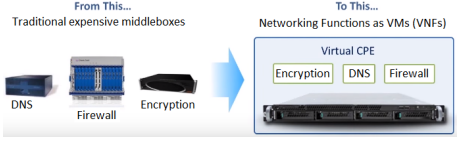
\includegraphics[width=1\textwidth]{2_2_2image}
    \caption{Network Function Virtualization}
    \label{fig:2_2_2image}
\end{figure}
\begin{itemize}
\item \textbf{Hardware Flexibility:} Because NFV uses regular Commercial-Off-The-Shelf (COTS)
hardware, network operators have the freedom to choose and build the hardware in
the most efficient way to suit their needs and requirements.
\item \textbf{Faster Service Life Cycle:} New network services can now be deployed more quickly,
in an on-demand and on-need basis, providing benefits for end users as well as the
network providers.
\item \textbf{Scalability and Elasticity:} New services and capacity-hungry applications keep network operators (especially cloud providers), on their toes to keep up with the fastincreasing demands of consumers.
\item \textbf{Increased Revenue:} The combination of introducing new services faster and existing
servers in a more dynamic fashion can jointly result in increased revenue.
\item \textbf{Reduced Capital Expenditures (CAPEX):} The use of industry-standard services,
increased hardware utilization and adoption of open source software results in reduced capital expenditures.
\item \textbf{Reduced Operational Expenditures (OPEX):} Automation and hardware standardization can substantially slash operational expenditures.
\item \textbf{Improved Customers' Satisfaction:} The combination of service agility and selfservice can result in greater customer satisfaction.
\item \textbf{Reduced Power Consumption and Complexity:} Efficiencies in space, power, and
cooling. Communications Service Providers (CSPs) may have finite physical space,
electrical power, and cooling capacity in a data center, so they will carefully select
equipment to efficiently consume those finite and/or costly resources. NFV provides
a better energy efficiency resulting from the consolidation of resources, as well as
their more dynamic utilization.
\end{itemize}
